
%(BEGIN_QUESTION)
% Copyright 2013, Tony R. Kuphaldt, released under the Creative Commons Attribution License (v 1.0)
% This means you may do almost anything with this work of mine, so long as you give me proper credit

\noindent
{\bf Lab Exercise}

\vskip 5pt

Your task is to completely disassemble, reassemble, and bench-set a pneumatically actuated control valve, preferably a Fisher (Emerson) E-body globe valve.  Also, you will build and troubleshoot a control loop to actuate that valve with an electronic 4-20 mA signal, using an I/P transducer as the signal converter between the electronic controller and the pneumatic valve.  

\underbar{Objective completion table:}

% No blank lines allowed between lines of an \halign structure!
% I use comments (%) instead, so that TeX doesn't choke.

$$\vbox{\offinterlineskip
\halign{\strut
\vrule \quad\hfil # \ \hfil & 
\vrule \quad\hfil # \ \hfil & 
\vrule \quad\hfil # \ \hfil & 
\vrule \quad\hfil # \ \hfil & 
\vrule \quad\hfil # \ \hfil & 
\vrule \quad\hfil # \ \hfil & 
\vrule \quad\hfil # \ \hfil \vrule \cr
\noalign{\hrule}
%
% First row
{\bf Performance objective} & {\bf Grading} & {\bf 1} & {\bf 2} & {\bf 3} & {\bf 4} & {\bf Team} \cr
%
\noalign{\hrule}
%
% Another row
Team meeting and prototype sketch & mastery & -- & -- & -- & -- & \cr
%
\noalign{\hrule}
%
% Another row
Control valve disassembly & mastery & -- & -- & -- & -- & \cr
%
\noalign{\hrule}
%
% Another row
Valve component identification & mastery & & & & & -- -- -- -- \cr
%
\noalign{\hrule}
%
% Another row
Torque wrench usage & mastery & & & & & -- -- -- -- \cr
%
\noalign{\hrule}
%
% Another row
Proper stroke length and bench-set & mastery & -- & -- & -- & -- & \cr
%
\noalign{\hrule}
%
% Another row
I/P calibration (with As-Found/As-Left) & mastery & -- & -- & -- & -- &  \cr
%
\noalign{\hrule}
%
% Another row
Circuit design challenge & mastery & & & & & -- -- -- -- \cr
%
\noalign{\hrule}
%
% Another row
Final loop diagram and system inspection & mastery & & & & & -- -- -- -- \cr
%
\noalign{\hrule}
%
% Another row
Demonstration of working system & mastery & -- & -- & -- & -- & \cr
%
\noalign{\hrule}
%
% Another row
Lab question: Instrument connections & proportional &  &  &  &  & -- -- -- -- \cr
%
\noalign{\hrule}
%
% Another row
Lab question: Commissioning & proportional &  &  &  &  & -- -- -- -- \cr
%
\noalign{\hrule}
%
% Another row
Lab question: Mental math & proportional &  &  &  &  & -- -- -- -- \cr
%
\noalign{\hrule}
%
% Another row
Lab question: Diagnostics & proportional &  &  &  &  & -- -- -- -- \cr
%
\noalign{\hrule}
%
% Another row
Lab clean-up & mastery & -- & -- & -- & -- &  \cr
%
\noalign{\hrule}
} % End of \halign 
}$$ % End of \vbox

The only ``proportional'' scoring in this activity are the lab questions, which are answered by each student individually.  A listing of potential lab questions are shown at the end of this worksheet question.  The lab questions are intended to guide your labwork as much as they are intended to measure your comprehension, and as such the instructor may ask these questions of your team day by day, rather than all at once (on a single day).

\vskip 10pt

{\bf It is essential that your team plans ahead what to accomplish each day.  A short (10 minute) team meeting at the beginning of each lab session is a good way to do this, reviewing what's already been done, what's left to do, and what assessments you should be ready for.  There is a lot of work involved with building, documenting, and troubleshooting these working instrument systems!}

As you and your team work on this system, you will invariably encounter problems.  You should always attempt to solve these problems as a team before requesting instructor assistance.  If you still require instructor assistance, write your team's color on the lab whiteboard with a brief description of what you need help on.  The instructor will meet with each team in order they appear on the whiteboard to address these problems.

$$\includegraphics[width=15.5cm]{i00769x01.eps}$$





\vfil \eject

\noindent
{\bf Lab Exercise -- team meeting and prototype sketch}

\vskip 5pt

An important first step in completing this lab exercise is to {\bf meet with your instructor} as a team to discuss safety concerns, team performance, and specific roles for team members.  If you would like to emphasize exposure to certain equipment (e.g. use a particular type of control system, certain power tools), techniques (e.g. fabrication), or tasks to improve your skill set, this is the time to make requests of your team so that your learning during this project will be maximized.

For example, if a team member lacks experience disassembling and reassembling mechanical devices, this lab exercise is an excellent opportunity to gain those skills.  It is {\it strongly} recommended that those team members with the least mechanical experience be the people to disassemble the valve while those with more experience merely supervise.  The team may work together in a more balanced fashion during re-assembly.  

Remember, the purpose of this lab exercise is not to complete it in the least amount of time, but rather for every team member to gain new knowledge and skill.  This is why tasks should not necessarily be assigned with {\it maximum efficiency} in mind as they would at a workplace, but rather with {\it maximum learning} in mind because this is a school.

\vskip 10pt

An absolutely essential step in completing this lab exercise is to work together as a team to {\bf sketch a prototype diagram} showing what you intend to build.  This usually takes the form of a simple electrical schematic and/or loop diagram showing all electrical connections between components, as well as any tubing or piping for fluids.  This prototype sketch need not be exhaustive in detail, but it does need to show enough detail for the instructor to determine if all components will be correctly connected for their safe function.

For example, if you intend to connect field devices to a PLC (Programmable Logic Controller), your prototype sketch must show how those devices will connect to typical input/output terminals on the PLC, where electrical power will be supplied, etc.  Prototype sketches need not show all intermediary connections between components, such as terminal blocks in junction boxes between the field device and the controller.

You should practice good problem-solving techniques when creating your prototype sketch, such as consulting equipment manuals for information on component functions and marking directions of electric current, voltage polarities, and identifying electrical sources/loads.  Use this task as an opportunity to strengthen your analytical skills!  Remember that you will be challenged in this program to do all of this on your own (during ``capstone'' assessments), so do not make the mistake of relying on your teammates to figure this out for you -- instead, treat this as a problem {\it you} must solve and compare your results with those of your teammates.

Your team's prototype sketch is so important that the instructor will demand you provide this plan before any construction on your team's working system begins.  {\it Any team found constructing their system without a verified plan will be ordered to cease construction and not resume until a prototype plan has been drafted and approved!}  Similarly, you should not deviate from the prototype design without instructor approval, to ensure nothing will be done to harm equipment by way of incorrect connections.  Each member on the team should have ready access to this plan (ideally possessing their own copy of the plan) throughout the construction process.  Prototype design sketching is a skill and a habit you should cultivate in school and take with you in your new career.





\vfil \eject

\noindent
{\bf Lab Exercise -- selecting components and planning the system}

\vskip 5pt

One of the most common problems students encounter when building any working system, whether it be a circuit on a solderless breadboard or an instrument loop spanning an entire room, is properly connecting and configuring all components.  An unfortunate tendency among most students is to simply start connecting parts together, essentially designing the system as they go.  This usually leads to improperly-connected components and non-functioning systems, sometimes with the result of destroying components due to those improper connections!

An alternative approach is to plan ahead by designing the system before constructing it.  This is easily done by sketching a diagram showing how all the components should interconnect, then analyzing that diagram and making changes before connecting anything together.  When done as a team, this step ensures everyone is aware of how the system should work, and how it should go together.  The resulting ``prototype'' diagram need not be complex in detail, but it should be detailed enough for anyone to see which component terminals (and ports) connect to terminals and ports of other devices in the system.  For example, your team's prototype sketch should be clear enough to determine all DC electrical components will have the correct polarities.  If your proposed system contains a significant amount of plumbing (pipes and tubes), your prototype sketch should show all those connections as well.

\vskip 10pt

Your first step should be identifying the model of control valve assigned to you, then finding appropriate documentation for it.  The Emerson website contains manuals for all the Fisher valves they sell, so your best resource is the Internet (and/or your Instrumentation Reference where a variety of instrument manuals have been downloaded for you).  Use this documentation to locate diagrams of the valve assembly as well as instructions.  Your instructor will check to see you have located and are familiar with the equipment manual(s).

\vskip 10pt

Your team's prototype sketch is so important that the instructor will demand you provide this plan before any construction on your team's working system begins.  {\it Any team found constructing their system without a verified plan will be ordered to cease construction and not resume until a prototype plan has been drafted and approved!}  Each member on the team should have ready access to this plan (ideally possessing their own copy of the plan) throughout the construction process.  Prototype design sketching is a skill and a habit you should cultivate in school and take with you in your new career.

\vskip 10pt

{\bf Planning a functioning system should take no more than an hour if the team is working efficiently, and will save you hours of frustration (and possible component destruction!).}





\vfil \eject

\noindent
{\bf Lab Exercise -- disassembling and re-assembling the valve}

\vskip 5pt

The {\it Lessons In Industrial Instrumentation} textbook has an Appendix section documenting the complete tear-down of a Fisher ``E-body'' sliding-stem globe valve.  You may want to use this as a guide in the disassembly of your team's valve.  Feel free to take your own digital photographs as you disassemble the valve, to better aid in your understanding of its function and to serve as a re-assembly guide.

A safety tip for disassembly is to make releasing spring tension your {\it first} step.  Back off the spring adjuster until it spins loosely, and then there should be no stored energy in the actuator spring to hurt you during disassembly.  If ever you are loosening a nut or bolt on the valve assembly and it seems to be ``stiff'' during most of the loosening process, you may very well have stored spring tension inside the valve that should be relieved before any further loosening is attempted.

You and your teammates should disassemble the control valve down to the last nut and bolt.  Use a coffee can or other container to place small items such as nuts, bolts, screws, brackets, clips, and O-rings.  Use a larger bucket or tub to hold major valve components during the disassembly and re-assembly processes.

\vskip 10pt

After disassembling the valve, each team member must properly identify a few key components of the valve (and their functions) as prompted by the instructor.

\vskip 10pt

When all team members have successfully passed the component identification test, the team is cleared to re-assemble the valve.  Be careful when doing so -- if components don't seem to fit smoothly, and/or require substantial force to put together, you are likely doing something incorrect.  Stop and re-evaluate your actions before you break something!

A helpful precaution to take when reassembling the valve body is to periodically move the valve stem by hand to ensure it continues to more freely and with full stroke (the stem should actually move just a bit {\it farther} than the rated stroke length, so long as the actuator remains unattached).  If the stem exhibits any sign of limited travel or binding, it is a sign something is wrong with the assembly, and you should disassemble it again to check your work.

Be sure to {\it cross-torque} all nuts and bolts arranged in a circular pattern (e.g. nuts on bonnet studs, diaphragm casing nuts and bolts): this means alternating sides when choosing the next nut/bolt to tighten.  Use a torque wrench to apply the amount of torque specified in the manufacturer's instruction manual, individually demonstrating this tool usage to the instructor.  Proper execution of the torque sequence will ensure the assembly will not be warped by uneven bolt stress.

\vskip 10pt

{\bf Common mistakes:}

\begin{itemize}
\item{} The most-mechanically-minded students doing all the work, when they should let their lesser-mechanically-inclined teammates do most of the disassembly.
\item{} Failing to consult documentation, especially with regard to the proper assembly of the stem packing.
\item{} Not organizing parts in containers.
\item{} Trying to hoist heavy valve components by yourself -- improper lifting techniques and lack of teamwork.
\item{} Using tools improperly: e.g. using adjustable wrenches when combination wrenches will do, using slip-joint and tongue-and-groove pliers instead of wrenches, using metal tools (hammer heads) to tap metal components out of place instead of softer tools such as the wooden handle of a hammer.
\item{} Not checking valve stem stroke periodically while reassembling valve body.
\end{itemize}

\vskip 10pt

{\bf Thoroughly disassembling a control valve should take no more than one full lab session (3 hours) if the team is working efficiently!  Identifying components and re-assembling the control valve may take more than one whole (3 hour) lab session.}


\vfil \eject

\noindent
{\bf Lab Exercise -- setting stroke length and bench-set pressure}

\vskip 5pt

The most complex step in the re-assembly process is properly setting both the stem stroke length and the bench-set pressure.  This step takes a bit of time to do, and it is easy to mis-understand, so be sure to budget plenty of time (at least an hour or two) to do it right.  Be sure to involve all team members in this procedure, as it is easy to mis-understand.

In a sliding-stem control valve, the length of the valve stem's travel (``stroke'') is determined by the coupling of the valve and actuator stems.  A {\it stem connector} couples these two stems together at just the right total stem length so that the valve plug ``bottoms out'' on the seat when at the 0\% position and the actuator ``tops out'' on the upper casing at the 100\% position.  In order to set the proper coupling point between the two stems, you will need some way to apply variable air pressures to the diaphragm actuator to move it between its extreme positions.  A small air pressure regulator connected to a compressed air supply works well for this purpose, and need not be precision.

\vskip 10pt

Consult the manufacturer's manual for your control valve's actuator to obtain step-by-step instructions for setting the valve spring tension (``bench set'') and also properly installing the stem connector (coupling).  The result, after correctly following the procedures, is that the valve's stem travel should exactly match what is shown on the travel indicator scale.  Your instructor will judge your team's proper assembly as such: the valve stem should just begin to move at slightly above the lower bench-set pressure, and reach full stroke just shy of the upper bench-set pressure value.  Decreasing the applied air pressure below the lower bench-set value or increasing the pressure above the upper bench-set value should produce no stem motion at all (i.e. the valve should mechanically ``bottom out'' and ``top out'' at these bench-set pressure values).

\vskip 10pt

Stroke length and bench-set are both crucial parameters for efficient and safe control valve operation.  Wrong stroke length can prevent the valve from fully opening (if the stems are coupled too far apart) and may even prevent it from fully closing (if the stems are coupled much too close together).  Proper stroke length ensures the valve will exhibit the engineered flow characteristics throughout its range of movement.  Improper bench set may result in insufficient seating pressure (if spring tension is too weak), causing the valve to pass fluid by when it should be fully closed.

\vskip 10pt

{\bf Common mistakes:}

\begin{itemize}
\item{} Not following the manufacturer's instructions {\it precisely}.
\end{itemize}






\vfil \eject

\noindent
{\bf Lab Exercise -- circuit design challenge}

\vskip 5pt

Connect an ``ice-cube'' relay to a low-voltage DC source as well as 120 volts AC so that a hand-operated switch will control the energization of a 120 VAC load.  All electrical connections must be made using a terminal strip (no twisted wires, crimp splices, wire nuts, spring clips, or ``alligator'' clips permitted), and the 120 VAC portion of the circuit must be fused for overcurrent protection.

This exercise tests your ability to properly interpret the ``pinout'' of an electromechanical relay, properly wire a switch to control a relay's coil, properly wire a load to the contacts of a relay, properly select NO/NC contacts on both the switch and the relay, and use a terminal strip to organize all electrical connections.

$$\includegraphics[width=15.5cm]{i00769x03.eps}$$

\vskip 10pt

The following components and materials will be available to you: assorted ``ice cube'' {\bf relays} with DC-rated coils and matching {\bf sockets} ; assorted pushbutton {\bf switches} ; {\bf terminal strips} ; lengths of {\bf hook-up wire} ; {\bf battery clips} (holders) ; 120 VAC {\bf power cord} with {\bf fuse assembly} ; 120 VAC {\bf lamp or other suitable load}.

\vskip 10pt

You will be expected to supply your own screwdrivers and multimeter for assembling and testing the circuit at your desk.  The instructor will supply the battery(ies) to power your circuit when you are ready to see if it works.  Until that time, your circuit will remain unpowered.

\vskip 20pt

\noindent
{\bf Load/switch status} (instructor chooses): \hskip 20pt \underbar{\hskip 20pt} On when pressed \hskip 10pt {\it or} \hskip 10pt \underbar{\hskip 20pt} Off when pressed

\vfil

Study reference: the ``Control Relays'' section of {\it Lessons In Industrial Instrumentation}.







\vfil \eject

\noindent
{\bf Lab Exercise -- building the system}

\vskip 5pt

The Instrumentation lab is set up to facilitate the construction of working instrument ``loops,'' with over a dozen junction boxes, pre-pulled signal cables, and ``racks'' set up with 2-inch vertical pipes for mounting instruments.  The only wires you should need to install to build a working system are those connecting the field instrument to the nearest junction box, and then small ``jumper'' cables connecting different pre-installed cables together within intermediate junction boxes.

After getting your prototype sketch approved by the instructor, you are cleared to build a hand-control system for it.  This will consist of a loop controller placed into ``manual'' mode to allow direct control over the valve's position.  There will be no transmitter installed in this loop -- just the valve and the I/P converter necessary to convert the controller's 4-20 mA output signal into a pneumatic signal to move the valve.  Feel free to use 1/4 inch plastic tubing for all pneumatic signal connections, and be sure not to exceed the rated supply pressure for the I/P (as documented in the I/P manual).

Your hand-control system needs to have a loop number, so all instruments within it may be properly labeled.  This loop number needs to be unique, so that another team does not label their instruments and tubes the same as yours.  One way to make your loop number unique is to use the equivalent resistor color-code value for your team's color in the loop number.  For example, if you are the ``Red'' team, your loop number could be ``2''. 

The controller itself should be labeled ``HC-'' because it is a ``hand'' controller, allowing a human operator manual control over the valve's position.

\vskip 10pt

{\bf Common mistakes:}

\begin{itemize}
\item{} Neglecting to consult the manufacturer's documentation for the I/P converter (e.g. how to connect pneumatic signal lines, how to calibrate it).
\item{} Improper pipe/tube fitting installation (e.g. trying to thread tube fittings into pipe fittings and vice-versa).
\item{} Over-tightening tube fittings (remember, no more than 1-1/4 turns when assembling, and no more than ``snug'' when re-making the connection!).
\item{} Students working on portions of the system in isolation, not sharing with their teammates what they did and how.  It is important that the whole team learns all aspects of their system!
\end{itemize}


\vfil \eject

\noindent
{\bf Lab Exercise -- documenting the system}

\vskip 5pt

Each student must sketch their own {\it loop diagram} for their team's system, following proper ISA conventions.  Sample loop diagrams are shown in the next question in this worksheet.  These loop diagrams must be {\it comprehensive} and {\it detailed}, showing every tube connection, every tube, range points, etc.  The principle to keep in mind here is to make the loop diagram so complete and unambiguous that anyone can follow it to see what connects to what, even someone unfamiliar with industrial instrumentation.  In industry, loops are often constructed by contract personnel with limited understanding of how the system is supposed to function.  The loop diagrams they follow must be so complete that they will be able to connect everything properly without necessarily understanding how it is supposed to work.

Every instrument and every signal tube in your loop needs to be properly labeled with an ISA-standard tag number.  An easy way to do this is to wrap a short piece of masking tape around each tube (and placed on each instrument) then writing on that masking tape with a permanent marker.  Although no industry standard exists for labeling signal tubes, a good recommendation is to label each tube with the tag number of the field instrument it goes to.  Thus, every length of tube in a hand control loop should be labeled ``HV-$x$'' (where ``$x$'' is the loop number).

When your entire team is finished drafting your individual loop diagrams, call the instructor to do an inspection of the loop.  Here, the instructor will have students take turns going through the entire loop, with the other students checking their diagrams for errors and omissions along the way.  During this time the instructor will also inspect the quality of the installation, identifying problems such as frayed wires, improperly crimped terminals, poor cable routing, missing labels, lack of wire duct covers, etc.  The team must correct all identified errors in order to receive credit for their system.  

After successfully passing the inspection, each team member needs to place their loop diagram in the diagram holder located in the middle of the lab behind the main control panel.  When it comes time to troubleshoot another team's system, this is where you will go to find a loop diagram for that system!

\vskip 10pt

{\bf Common mistakes:}

\begin{itemize}
\item{} Forgetting to label all signal tubes (see example loop diagrams).
\item{} Forgetting to label all field instruments with their own tag names (e.g. HY-83 for the I/P transducer).
\item{} Forgetting to put your name on the loop diagram!
\item{} Basing your diagram off of a team-mate's diagram, rather than closely inspecting the system for yourself.
\item{} Not placing loop sheet instruments in the correct orientation (field instruments on the left, control room instruments on the right).
\end{itemize}

\vskip 10pt

{\bf Creating and inspecting accurate loop diagrams should take no more than one full lab session (3 hours) if the team is working efficiently!}





\vfil \eject

\noindent
{\bf Lab Exercise -- I/P calibration}

\vskip 5pt

Each team must calibrate their I/P transducer for a range appropriate to their control valve's actuator pressure range (usually 3-15 PSI).  As in all cases where an instrument must be calibrated, you will need to check the instrument's response against one or more {\it standards}.  In this case, the ideal standard to use for measuring the I/P output pressure is a {\it test gauge}, and the ideal standard to use for establishing the 4-20 mA current signal into the I/P is a {\it loop calibrator} set to ``source'' current.

$$\includegraphics[width=15.5cm]{i00769x02.eps}$$

Read the manufacturer's documentation on the I/P transducer for details on how to calibrate it.  Like an analog measuring instrument, the procedure will involve trial-and-error applications of LRV and URV input signal values, adjusting the ``zero'' and ``span'' screws of the I/P until it tracks accurately at those two points.  Note that the zero and span screw adjustments on most I/P converters are interactive: adjusting the span will affect the zero, necessitating a lot of back-and-forth applications of LRV and URV, zero screw turning and span screw turning.

\filbreak

Document the accuracy of your I/P's calibration before and after adjustment in these tables, at five different points throughout its sensing range.  The ``Applied'' current is the amount of electric current you apply to the I/P's input using a loop calibrator, and the ``Output'' signal is the amount of air pressure output by the I/P (the 3-15 PSI range):

\vskip 10pt

{\bf As-Found calibration table}

% No blank lines allowed between lines of an \halign structure!
% I use comments (%) instead, so that TeX doesn't choke.

$$\vbox{\offinterlineskip
\halign{\strut
\vrule \quad\hfil # \ \hfil & 
\vrule \quad\hfil # \ \hfil & 
\vrule \quad\hfil # \ \hfil & 
\vrule \quad\hfil # \ \hfil \vrule \cr
\noalign{\hrule}
%
% First row
Applied pressure & Output signal (actual) & Output signal (ideal) & Error (\% of span) \cr
%
\noalign{\hrule}
%
% Another row
 &  &  & \cr
%
\noalign{\hrule}
%
% Another row
 &  &  & \cr
%
\noalign{\hrule}
%
% Another row
 &  &  & \cr
%
\noalign{\hrule}
%
% Another row
 &  &  & \cr
%
\noalign{\hrule}
%
% Another row
 &  &  & \cr
%
\noalign{\hrule}
} % End of \halign 
}$$ % End of \vbox

\vskip 10pt

{\bf As-Left calibration table}

% No blank lines allowed between lines of an \halign structure!
% I use comments (%) instead, so that TeX doesn't choke.

$$\vbox{\offinterlineskip
\halign{\strut
\vrule \quad\hfil # \ \hfil & 
\vrule \quad\hfil # \ \hfil & 
\vrule \quad\hfil # \ \hfil & 
\vrule \quad\hfil # \ \hfil \vrule \cr
\noalign{\hrule}
%
% First row
Applied pressure & Output signal (actual) & Output signal (ideal) & Error (\% of span) \cr
%
\noalign{\hrule}
%
% Another row
 &  &  & \cr
%
\noalign{\hrule}
%
% Another row
 &  &  & \cr
%
\noalign{\hrule}
%
% Another row
 &  &  & \cr
%
\noalign{\hrule}
%
% Another row
 &  &  & \cr
%
\noalign{\hrule}
%
% Another row
 &  &  & \cr
%
\noalign{\hrule}
} % End of \halign 
}$$ % End of \vbox

When finished calibrating your I/P converter, be sure to place a calibration tag on it showing the range and the date it was calibrated.  The first page of this lab exercise has cut-out calibration tags you may tape to the I/P for this purpose.

The accuracy of your calibration will be checked by the instructor while installed in the loop, setting the hand controller's output to various levels and checking the valve stem position for correspondence.  It should be noted that I/P transducers are not typically ``precision'' instruments like process transmitters, and as such you may find substantial variations in calibration resulting from modest changes in supply air pressure and/or mounting position.

\vskip 10pt

{\bf Common mistakes:}

\begin{itemize}
\item{} Applying excessive force to I/P adjustments.  This is a delicate mechanism!  As such, it should {\it not} require forceful adjustment!!  If you have to {\it force} something, you're probably doing it wrong.
\item{} Improper supply air pressure to the converter (see the manual for supply air pressure specifications)
\item{} Improper pipe/tube fitting installation (e.g. trying to thread tube fittings into pipe fittings and vice-versa).
\item{} Neglecting to place a calibration tag on the I/P converter after calibrating it.
\end{itemize}








\vskip 10pt

\vfil \eject

\noindent
{\bf Lab questions}

\begin{itemize}
\item{} {\bf Instrument connections}
\item{} Determine correct wire connections between instruments to create a working 4-20 mA loop circuit, based on diagrams of instruments with terminals labeled
\item{} Correctly determine all electrical sources and loads, as well as all voltage polarities and current directions in a 4-20 mA loop circuit, based on diagrams of instruments with terminals labeled
\end{itemize}

\filbreak

\begin{itemize}
\item{} {\bf Commissioning and Documentation}
\item{} Identify alternative valve actuators (other than pneumatic diaphragm)
\item{} Identify the major components of a rotary ball control valve from a diagram
\item{} Explain the function of valve stem packing, and how to change it
\item{} Explain how to adjust the compression on a valve's stem packing
\item{} Explain how to properly set valve stroke length and bench-set pressure
\item{} Explain the significance of properly setting valve stroke length and bench-set pressure
\end{itemize}

\filbreak

\begin{itemize}
\item{} {\bf Mental math} (no calculator allowed!)
\item{} Convert between different pressure units, without relying on the use of a reference for conversion factors (i.e. you must commit the major conversion factors to memory)
\item{} Calculate the correct pneumatic output pressure (PSI) from an I/P transducer given an applied current (mA) signal input and a specified range (e.g. 4-20 mA input ; 3-15 PSI output)
\item{} Calculate the applied input current (mA) to an I/P transducer given a measured pneumatic output pressure (PSI) and a specified range (e.g. 4-20 mA input ; 3-15 PSI output) 
\item{} Calculate the percentage of span error for an I/P transducer given a calibration range and an As-Found calibration table 
\item{} Calculate force generated by a diaphragm or piston actuator given diameter and applied fluid pressure in units of PSI
\end{itemize}

\filbreak

\begin{itemize}
\item{} {\bf Diagnostics}
\item{} Determine whether or not a given diagnostic test will provide useful information, given a set of symptoms exhibited by a failed system
\item{} Identify at least two plausible faults given the results of a diagnostic test and a set of symptoms exhibited by a failed system
\item{} Propose a diagnostic test for troubleshooting a failed system and then explain the meanings of two different test results
\end{itemize}



\vfil \eject

\noindent
{\bf Lab Exercise -- decommissioning and clean-up}

\vskip 5pt

The final step of this lab exercise is to decommission your team's entire system and re-stock certain components back to their proper storage locations, the purpose of which being to prepare the lab for the next lab exercise.  Remove your system documentation (e.g. loop diagram) from the common holding area, either discarding it or keeping it for your own records.  Also, remove instrument tag labels (e.g. FT-101) from instruments and from cables.  Perform general clean-up of your lab space, disposing of all trash, placing all tools back in their proper storage locations, sweeping up bits of wire off the floor and out of junction boxes, etc.

\vskip 10pt

\indent
{\bf Leave the following components in place, mounted on the racks:}

\begin{itemize}
\item{} Large control valves and positioners
\item{} I/P transducers
\item{} Large electric motors
\item{} Large variable-frequency drive (VFD) units
\item{} Cables inside conduit interconnecting junction boxes together
\item{} Pipe and tube fittings (do not unscrew pipe threads)
\item{} Supply air pressure regulators
\end{itemize}

\vskip 10pt

\indent
{\bf Return the following components to their proper storage locations:}

\begin{itemize}
\item{} Sensing elements (e.g. thermocouples, pH probes, etc.)
\item{} Process transmitters
\item{} ``Jumper'' cables used to connect terminal blocks within a single junction box
\item{} Plastic tubing and tube fittings (disconnect compression-style tube fittings)
\item{} Power cables and extension cords
\item{} Adjustment (loading station) air pressure regulators
\end{itemize}

\vskip 10pt

Finally, you shall return any control system components to their original (factory default) configurations.  This includes controller PID settings, function block programs, input signal ranges, etc.



\underbar{file i00769}
%(END_QUESTION)





%(BEGIN_ANSWER)


%(END_ANSWER)





%(BEGIN_NOTES)

\noindent
{\bf Loop diagrams / inspections:}

I strongly recommend checking off students' loop diagrams while you inspect their loop (checking for secure wiring, proper tubing, good conduit installation, etc.) with them.  Have all team members take you on a ``tour'' of their completed loop, with each team member explaining a different portion of the loop you select while using their own loop diagram as a guide.  While a student is explaining their section of the loop, you can check the other students' loop diagrams for accuracy.  This not only saves time by consolidating the tasks of loop inspection and loop diagram verification, but it also ensures students can actually relate their loop diagrams to the loop they have built and articulate that understanding to you.

\vskip 10pt

\goodbreak

{\bf Troubleshooting fault ideas:}

\begin{itemize}
\goodbreak
\item{} Connect instrument tubes to wrong port (construction fault)
\item{} Replace I/P restrictor with pre-faulted (plugged) unit (high output fault)
\item{} Replace I/P relay with pre-faulted unit (low or high output fault)
\item{} Turn supply air pressure down well below 15 PSI (low output fault)
\item{} Strip wire at terminal, then insert insulated wire end under terminal and tighten (open wire fault)
\item{} Cut signal cable somewhere in mid-conduit (open wire fault)
\item{} Push a thumbtack through the cable somewhere in mid-conduit (shorted wire fault)
\item{} Wire instrument cable conductors backward (construction fault)
\item{} Plug tube connections using portion of foam earplug stuffed into tube fitting (slow response fault)
\item{} Close air supply block valve and leave safety tag hanging on it (operator/technician error)
\item{} Give students wrong loop diagram (documentation fault)
\end{itemize}















\vfil \eject

\noindent
{\bf Lab questions}

\vskip 20pt

\item{$(1)$} Sketch the necessary wire connections allowing the loop calibrator to exert control over the valve in this diagram, and also identify the proper mode ({\it Read}, {\it Source}, or {\it Simulate}) to set the calibrator:

$$\includegraphics[width=15.5cm]{i00769x05.eps}$$

\vskip 40pt

\item{$(2)$} Describe the proper precedure for setting both valve stroke length and bench-set pressure on a sliding-stem control valve.

\vskip 20pt

\filbreak

\item{$(3)$} Calculate the amount of force generated by a 14 inch diameter valve actuator diaphragm, with an applied air pressure of 30 PSI.

\vskip 40pt

\item{$(4)$} Control valve TV-37 has failed in the closed position and refuses to open.  A voltmeter reading between terminals 3 and 4 shows 3.5 volts.  Identify one possible fault, as well as one impossible fault, with regard to these symptoms.  Be specific in your identification: both the location (which component) and nature (e.g. open, shorted, plugged) of each fault.

$$\includegraphics[width=15.5cm]{i00769x04.eps}$$















\vfil \eject

\noindent
{\bf Lab questions}

\vskip 20pt

\item{$(1)$} Sketch the necessary wire connections allowing the Honeywell controller to exert manual control over the valve in this diagram:

$$\includegraphics[width=15.5cm]{i00769x05.eps}$$

\vskip 40pt

\item{$(2)$} Explain the significance of properly setting valve stroke length and bench-set pressure on a sliding-stem control valve.

\vskip 20pt

\filbreak

\item{$(3)$} Calculate the percentage of span error for an I/P transducer given a calibrated range of 3-15 PSI, if we know it outputs 11.85 PSI of air pressure at an input current of 16.00 mA.

\vskip 40pt

\item{$(4)$} Control valve TV-37 has failed in the wide-open position and refuses to close at all.  A voltmeter reading between terminals 3 and 4 shows 0.8 volts.  Identify one possible fault, as well as one impossible fault, with regard to these symptoms.  Be specific in your identification: both the location (which component) and nature (e.g. open, shorted, plugged) of each fault.

$$\includegraphics[width=15.5cm]{i00769x04.eps}$$




%INDEX% Lab exercise, control valve rebuild

%(END_NOTES)


